% CpSc 855 - Final paper
% Takumi Bolte & Dan Welch - Spring 2014.
\documentclass{sig-alternate}
%\usepackage{flushend}		% For automatically balancing reference columns

\begin{document}
\conferenceinfo{Clemson 2014}{7th Clemson University Mini-Conference on Embedded Network Systems}
\title{An Extensible Approach to Verification of Embedded Network Systems*}

%Re-evaluating Verification of Embedded Network Systems:
%An Extensible Approach to Verification of Embedded Network Systems*}
\numberofauthors{2}
\author{
\alignauthor
%author
Daniel Welch\\
\affaddr{School of Computing, Clemson University}\\
\affaddr{Clemson, South Carolina, 29634}\\
\email{\texttt{\large{\{dtwelch\}@clemson.edu}}}
%author
\alignauthor
Takumi Bolte\\
\affaddr{School of Computing, Clemson University}\\
\affaddr{Clemson, South Carolina, 29634}\\
\email{\texttt{\large{\{tbolte\}@clemson.edu}}}
}

\maketitle
\begin{abstract}

In this paper we present a flexible means of specifying and verifying the correctness of software for embedded network systems. Our approach uses RESOLVE, an imperative, component based programming and mathematical specification language, to verify the functional correctness of TinyOS applications. In doing so, we enrich the work originally presented in \cite{regula:2010} with the following: A model view controller (MVC) based implementation of a RESOLVE to C translator, a dynamic memory allocation scheme tailored towards embedded systems running the code generated by our tool, and the addition of a new language keyword that enables users to pair custom RESOLVE specifications with `externally' implemented (non RESOLVE) realizations. We demonstrate these additions with a revised version of the LED template originally presented in \cite{regula:2010} that showcases some of the more recent mathematical developments in ``string theory" (resolve's mathematical string library) as well as verification of a simple enhancement for Leds template that includes preliminary generation of performance profile characteristics.
\end{abstract}

\category{D.2.8}{Software Engineering and Data Communication}{Verification}[VCs, automated proving, modular software]
\terms{Reliability, Verification, Languages, Networks}
\keywords{automation, components, formal methods, specification, verifying compiler, embedded networks, wireless sensing}

\section{Introduction}
\label{sec:intro}
Within little more than a decade, the area of embedded network systems and wireless sensing has exploded in popularity within industry and academia alike. Tempering however this extremely quick rise in popularity is the inherent difficulties in developing applications that function as intended in low power, event-driven environments. In response to these difficulties, a variety of tools and languages have been put forth  to help ease the burden on developers. On one end of this effort are languages such as NesC (Network embedded sensor C) which strive to minimize concurrency issues and other common sources of error by hiding libraries of pre-written drivers underneath hierarchies of software and interface level abstractions. The other end is largely comprised of simulation tools such as TOSSIM, Cooja, and Arora that make use of high-fidelity simulations of mote network and hardware behavior to model networks offline in controlled, repeatable environments.

Though these and other tools have indeed proven invaluable in allowing users to test and reason about event-driven code prior to deployment, they remain incapable of providing complete assurance that code will behave as expected when deployed in the field. 

In this paper, we approach this problem by using RESOLVE (Reusable Software Language with Verification) [CITE] [CITE] [CITE] as means of specifying, writing, and ultimately verifying proposed embedded code at a high level, then present a technique of translating this verified code down into lower level, embedded-platform friendly C.  

Our choice to use RESOLVE as a language and verification frontend stems from the language's well acknowledged characteristics [CITE] that emphasize the following:
\begin{itemize}
\item \textbf{Modularity} At the language level, a strict separation of concerns is enforced between module specifications and client implementations. Thus, for any one particular specification, there can be any number of interchangeable implementations. This separation is ideal considering that many embedded applications are composed in similar fashion: Various drivers oftentimes provide a fixed set of operations, but have many distinct implementations that vary from platform to platform, vendor to vendor.

\item \textbf{Mathematical flexibility} RESOLVE offers a flexible mathematical typing system that allows users to either draw from a library of preexisting mathematical units when writing specifications, or create their own. 

\end{itemize}

This paper aims to leverage RESOLVE's mathematical flexibility of and component based design principles to the challenge of formally verifying an LED driver for the Telos motestack family.

We discuss this challenge in three parts. In the first, we provide both a short overview of the Telos family mote platform -- including a description of the LEDs driver which we later specify, verify, and translate -- as well as a short overview of the RESOLVE language itself. In the second section, we provide revised specifications for the LED drivers as well as a single enhancement on these drivers. This is followed by a review discussing the results of verification along with a review of some verification conditions generated by the compiler involving preliminary results for performance characteristics of enhancements. In the third and final section of the paper, we discuss the tool itself -- providing implementation details as well as a discussion of how this iteration of the tool differs from that originally detailed in \cite{regula:2010}. Finally, we conclude by discussing tool improvements and directions for future research.
\begin{figure*}
\centering
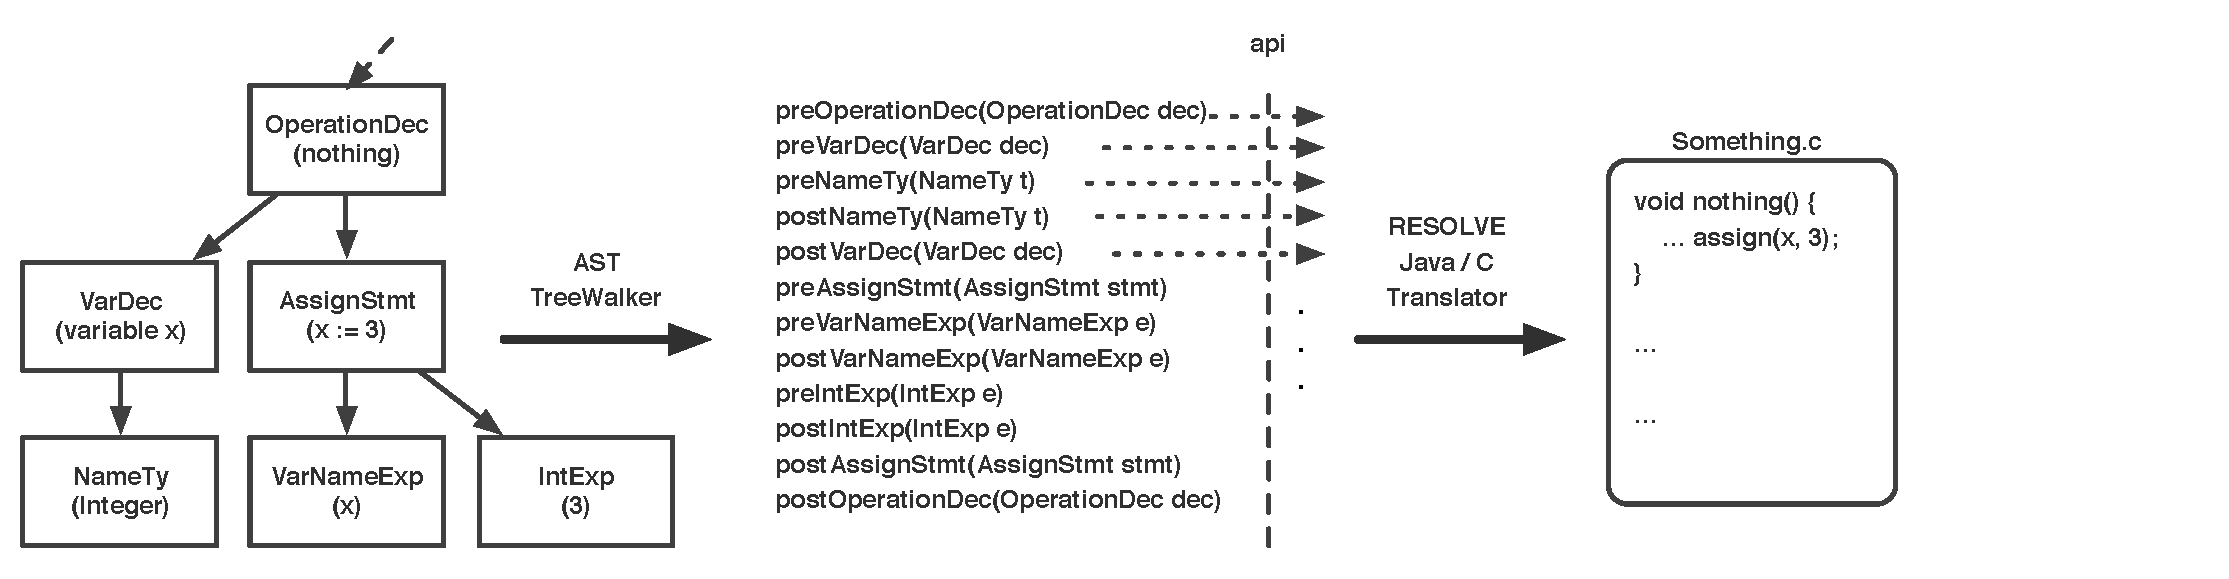
\includegraphics[scale=.55]{figs/ast_traversal.pdf}
\caption{An AST of a RESOLVE operation and its corresponding AST treewalker call sequence.}
\end{figure*}
\label{fig:ast}
\section{A model for c translation}

One of the primary challenges in translating from RESOLVE to C is finding a suitable C representation for each RESOLVE module and the constructs allowable in each. As we are dealing with an environment where functional correctness is a primary concern, it is especially important that the code generated represents as closely as possible the original RESOLVE source. In an effort to make such considerations, at the highest level, our tool outputs code specifically tailored to one of three distinct RESOLVE module types.

\begin{description}
\item [Concepts]
To model as closely as possible the role of a concept module, our tool produces a single .h file that contains structures for each parameter to a concept, pointers corresponding to the abstract types defined by the concept, as well as set of function pointers for each of the methods provided by the original RESOLVE concept.

\item [Realizations] 
Referring to both enhancement realizations as well as concept realizations, these are translated into a .h/.c pair. The header portion of this pair contains function declarations for the creation and destruction of a ``Realization\_Specific" facility. Elements of this facility are accessible only through a concept interface. The .c file has 5 sections:

\item [Facilities]


\end{description}




The representation of objects make use of a special 

\section{Implementation}
Development of the tool presented here can be logically partitioned into two phases: The tool that performs the actual translation from RESOLVE to C, and a separate tool that is called by the generated code that is responsible for allocating appropriate amounts of memory on the motestack without needing to resort to static allocation. 

\subsection{Translation AST walking}
Translation is performed over the course of a traversal of RESOLVE's abstract syntax tree (AST). The traversal mechanism used is a dervivative of the visitor pattern that provides a SAX-dom style pre-post traversal over all nodes in the tree. Thus, for any given node present, a total of two visits occur: One corresponding to the node being `hit' during the pre traversal stage, and one for the post. 

To make this more concrete, consider the following dummy operation.

\begin{verbatim}
operation nothing() procedure;
    var x : Integer;
    x := 3;
end nothing;
\end{verbatim}

Shown in Figure \ref{fig:ast} is the AST representation of operation \texttt{nothing}. Here, language constructs are represented as labeled boxes, while the actual traversal over these constructs -- and the order in which it is performed -- is communicated on the right via the call stack. Each of these calls are received in the translator in the order in which they are visited within the tree. It is up to the client (in this case, the author of the C-translator) to decide which of these methods they wish to override and perform custom actions within. 

We feel this particular traversal pattern lends itself well to the this application for the following reasons:

\begin{itemize}
\item A visit method for a construct provides a convenient encapsulation of all the logic required to translate RESOLVE construct $x$ to an appropriate C construct $y$.

\item Overriden visit methods apply to every instance of a construct -- meaning RESOLVE's C translator requires few (if any) loops, as the walk itself serves as the method of iteration.

\item Finally, only the visit methods for the constructs we currently wish to process need to be overridden. This makes it especially easy to tweak and optimize the size of the codebase for the C translator.
\end{itemize}

\subsection{Translation output}
Output of translated code is done using \textit{Stringtemplate} -- a third-party tool written in Java that allows users to define parameterizable templates. Like the name suggests, a template is simply ``a document with holes" that the user choses when and how to fill. 

An example of a template for a function/operation definition might look like the following:

\begin{verbatim}
function_def(modifier, type, name, params, 
                               vars, stmts) ::= <<
<modifier> <type> <name> (<params; sep = ", ">) {
    <vars; sep = "\n">
    <stmts; sep = "\n">
}>>
\end{verbatim}

Words enclosed in \texttt{<..>} signifies an attribute passable to the template and indicates where it will be positioned. It is entirely up to the user to define which attributes they wish to fill in, and at what level of granularity they wish to compose their templates. For example, the user might opt to fill-in and pass the \texttt{parameter(..)} template shown below to the \texttt{params} attribute, or, alternatively, a simple string.

\begin{verbatim}
parameter(type, name) ::= "<type> <name>"
\end{verbatim}

In the context of language translation, these templates when stored on a stack and manipulated over the course of the AST traversal, simplify the task of producing arbitrarily complicated, nested blocks of C output. For instance, upon visiting \texttt{preOperationDec}, a \texttt{function\_def} template can be instantiated by the client and pushed onto a global translation stack with its \texttt{name}, return \texttt{type}, and \texttt{modifier} attributes filled in. As \texttt{preOperationDec}'s children get visited, the \texttt{function\_def} template currently at the top of the stack receives similarly constructed parameter, variable, and statement templates from the corresponding child nodes. Upon reaching \texttt{postOperationDec}, we can be assured that the function has been completely filled in -- assuming the user implemented the visit methods for the children.

Hence, the only work being done within visit methods themselves is forwarding appropriate information from tree-nodes to an externally defined template. This allows us to exploit (in shameless design pattern parlance) a strict model view controller (MVC) separation in our translator's codebase between the mechanism that does the AST visiting (controller), the tree nodes from which we're adding information to templates (model), and the external file containing all available C language templates (view).




%One of the primary allures of this approach to translation is that that adheres to strict MVC design principles -- meaning that all output logic is distinctly separated from translation related logic. 

%We take advantage of these pre post methods using templates and simple stack to implement 


%Going even further, we demonstrate this by showing the steps taken to translate a simple operation declaration \texttt{nothing} to C.

% for each construct to remain encapsulated within that method, and (almost) completely eliminates the need for complex loop or iteration mechanisms. 


%This particular traversal pattern lends itself well to the language translation challenge (specifically source to source) where the pre methods align naturally with beginning of a construct, and conclude with its corresponding post method.  For instance, in the case above, this allows us, upon receiving a callback for In an effort to keep logic implementing our translator distinct and separate from the output language, we used a model view controller framework for implementing 

%To illustrate this, consider once again facility \texttt{DoNothing}.


\subsection{Garbage collection}



a source to source translator which, given a resolve component, outputs a C representation of that component. 
 
%To date there have been very few practical applications of verifiable code on physical media. 

\section{Acknowledgements}

Special thanks to Mike Kabanni and Mark Todd whose initial contributions and suggestions for the model of C translation paved the way to this paper. 

%Open up the .tex file and compile it using Latex (Shift+Apple+L) then compile it using Bibtex (Shift+Apple+B)
\bibliographystyle{unsrt}
\bibliography{sigproc}
\end{document}